% set margins and font
\documentclass[12pt,letterpaper]{article}
\usepackage[margin=1in]{geometry}
\usepackage{helvet}
\renewcommand{\familydefault}{\sfdefault}

% amsmath and amssymb packages, useful for mathematical formulas and symbols
\usepackage{amsmath,amssymb}

% citation manager and bibliography formatting
\usepackage[english]{babel}
\usepackage[square,numbers]{natbib}
\bibliographystyle{unsrt}
\setlength{\bibsep}{11pt}

% include images
\usepackage{graphicx}
\usepackage[font=footnotesize,labelfont=bf]{caption} % reduce default caption font size

% Use Unicode characters when possible
\usepackage[utf8x]{inputenc}

% array package and thick rules for tables
\usepackage{array}

% Remove comment for double spacing
\usepackage{setspace} 
\linespread{2}

% text symbol package
\usepackage{textcomp}

% insert pdf pages
\usepackage{pdfpages}

\begin{document}

% AFTER YOU DEFEND YOU PUT YOUR CERTIFICATE HERE
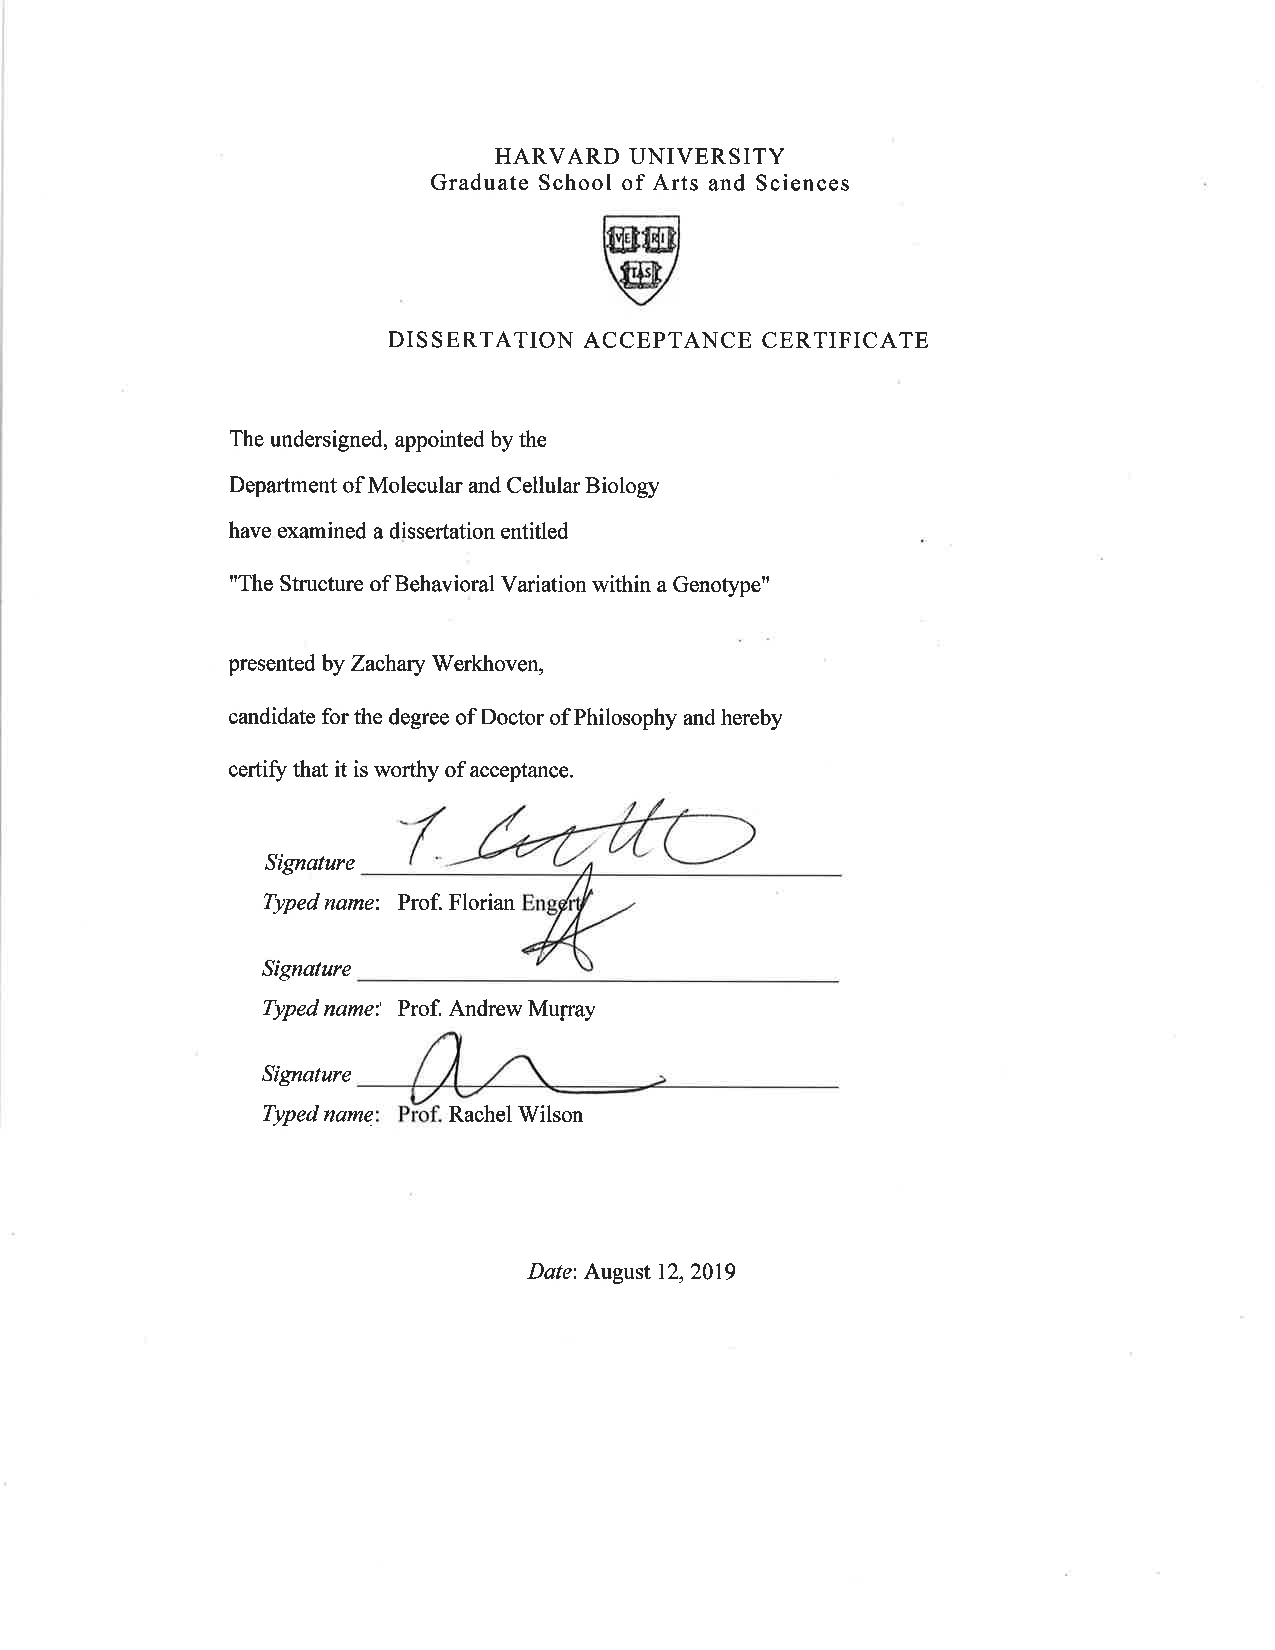
\includepdf[page=1]{defense_certificate.pdf}

% Harvard REQUIRES you to insert an empty page here
\vspace*{0.2in}
\thispagestyle{empty} 
\clearpage

% Harvard REQUIRES roman numeral page numbering for these header pages
% begin roman numeral page numbering
\pagenumbering{roman}

% TITLE PAGE
\begin{titlepage}
	\centering
	\vspace{1cm}
	{\scshape \large The Structure of Behavioral Variation Within a Genotype\par}
	\vspace{1.0cm}
	A dissertation presented\par \vspace{0.35cm}
	by\par \vspace{0.35cm}
	Zachary Werkhoven\par \vspace{0.35cm}
	to\par \vspace{0.35cm}
	The Department of Molecular and Cellular Biology\par \vspace{0.35cm}
	in partial fulfillment of the requirements\par \vspace{0.35cm}
	for the degree of\par \vspace{0.35cm}
	Doctor of Philosophy\par \vspace{0.35cm}
	in the subject of\par \vspace{0.35cm}
	Molecular and Cellular Biology\par \vspace{0.35cm}
	\vfill
	Harvard University\par
	Cambridge, Massachusetts\par
	August 2019
	\vfill
\end{titlepage}
\clearpage
% END TITLE PAGE

% COPYRIGHT PAGE
\topskip0pt
\vspace*{\fill}
    \begin{center}
    \textcopyright \hspace{0.01in} 2019 Zachary Werkhoven
    \end{center}
    \begin{center}
    All Rights Reserved.
    \end{center}
    \thispagestyle{empty}       % set page numbering style to blank
\vspace*{\fill}
\clearpage
% END COPYRIGHT

% ABSTRACT TITLE AND HEADER
\noindent Advisor: Ben de Bivort \hfill Zachary Werkhoven
\newline
\vspace{-1.2cm}
\setcounter{page}{3}
\begin{center}\large The Structure of Behavioral Variation Within a Genotype \newline \small \textbf{Abstract}\end{center}
\newline

% ABSTRACT BODY
Abstract body text goes here...
\clearpage
% END ABSTRACT BODY


% TABLE OF CONTENTS
% (this will auto-populate from \section and \subsection)
\tableofcontents
\clearpage


% INTRODUCTION chapter title page
\begin{center}
    \Large\section{Introduction}
    \pagenumbering{arabic}      % switch page numbering to arabic numerals
    \thispagestyle{empty}       % set page numbering style to blank
    \clearpage
\end{center}

 % reset the page counter to 1 (Harvard REQUIRES page count to start here)
\setcounter{page}{1}       
\subsection{What is Behavioral Covariation?}

Intro subsection text ... Example sentence with citations \cite{Goodman_IsoGrasshopers_1978,Chou_jcomp_2010}. And another for good measure... \cite{Linneweber_A_2019}

\subsection{Drosophila as a Model of Individual Behavioral Variation}

Intro subsection text...

\subsection{Neural Circuit Bottlenecks as a Potential Source of Behavioral Covariation}

Intro subsection text...

\subsection{Do Behaviors Evolve Independently or as Sets of Behaviors?}

Intro subsection text...

\subsection{Systematic Behavioral Profiling}

Intro subsection text...

% --- CHAPTER TWO --- %
% insert chapter title on its own page
\clearpage
\begin{center}
    \Large\textbf{Chapter 2}
    \thispagestyle{empty}       % set page numbering style to blank
    \clearpage
\end{center}

\section{MARGO: a Platform for High-Throughput Individual Ethology}

\subsection{Overview}

High level overview of chapter 2 and background info...

\subsection{Existing Animal Trackers}

Chapter 2 subsection text...

\subsection{Design Goals}

Chapter 2 subsection text...

% EXAMPLE FIGURE 
\begin{figure}[t!]
    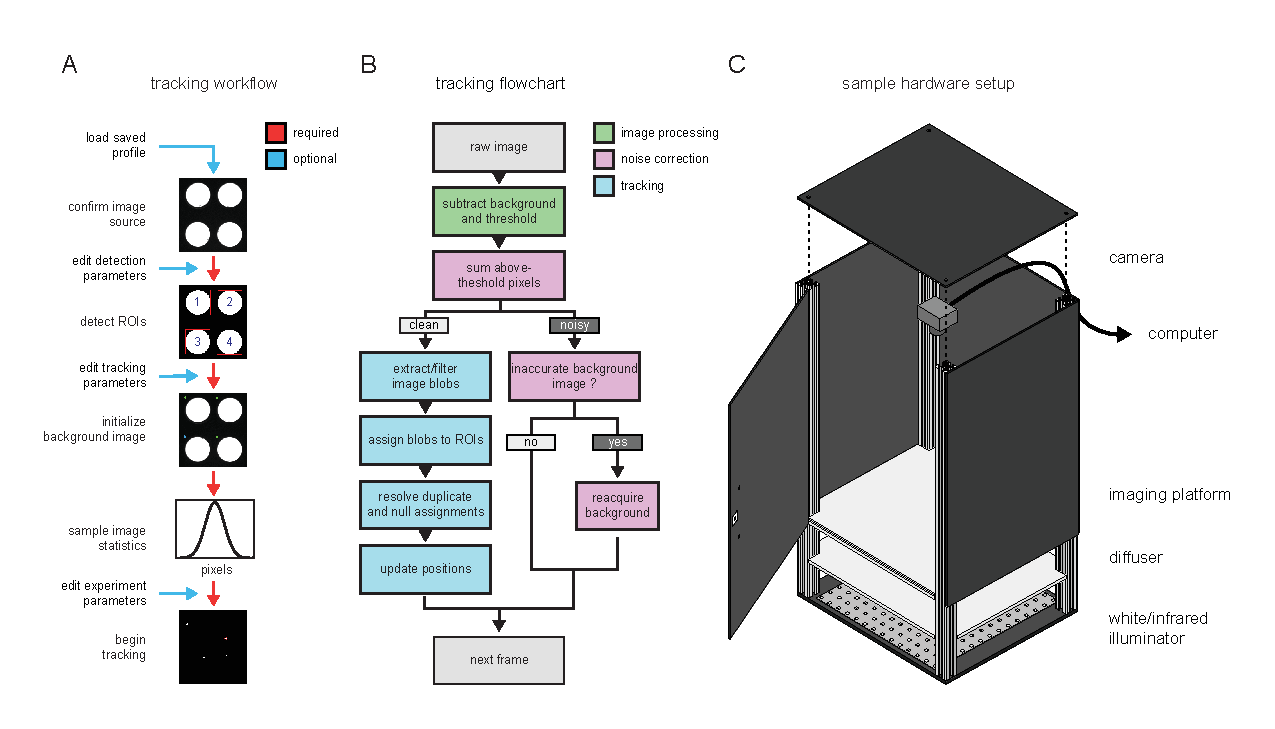
\includegraphics[width=\textwidth]{../figures/chapter_2/fig_2-1.pdf}
    \vspace{.1in}
    \caption*{\textbf{Figure 2.1} Example figure and tips -- A) Your figure numbers should follow the format of Figure chapter#.figure#. B) Set width equal to textwidth. C) Specify position as [t!] to insert at page top.}
\end{figure}

\subsection{Tracking Workflow}

Chapter 2 subsection text...

\subsection{Accuracy and Noise Robustness}

Chapter 2 subsection text...

\subsection{Application for High-throughput Behavioral Screens}

Chapter 2 subsection text...

\subsection{Platform Customization and Versatility}

Chapter 2 subsection text...

% example subsection heading that is NOT counted in the table of contents
\subsection*{\textit{Example subsection heading that is NOT counted in the table of contents}}

Chapter 2 subsection text...

\subsection{Utility of MARGO for the Scientific Community}

Chapter 2 subsection text...

% --- CHAPTER THREE - TITLE PAGE --- %
\clearpage
\begin{center}
    \Large\textbf{Chapter 3}
    \thispagestyle{empty}       % set page numbering style to blank
    \clearpage
\end{center}

% --- CHAPTER THREE --- %
\section{Decathlon Screen of Individual Behavioral Variation}

\subsection{Background}

High level overview of chapter 3 and background info...


\subsection{Project Goals}

Chapter 3 subsection text...


\subsection{Screen Results}

Chapter 3 subsection text...


\Subsection{Response of Clumpiness and Switchiness to Thermogenetic Manipulation}

Chapter 3 subsection text...


\subsection{Transcriptomic Profiling of Decathlon Individuals}

Chapter 3 subsection text...


\subsection{Meta-analysis of Fruit Fly Behavioral Covariation}

Chapter 3 subsection text...


%%%%%%%%%%%%%%%%%%%%%%%%%%%%%%%%%%%%%%%%%%%%%%%%%%%%%%%%%%%%%%%%%%%%%%%%%%%%%%%%%%%%%%%%
% --- CHAPTER FOUR - TITLE PAGE --- %
\clearpage
\begin{center}
    \Large\textbf{Chapter 4}
    \thispagestyle{empty}       % set page numbering style to blank
    \clearpage
\end{center}

% --- CHAPTER 4 --- %
\section{Conclusions and Future Directions}


\subsection{Structure of Behavioral Correlation in the Decathlon}

High level recap on the entire thesis up to this point...


\subsection{Remarks on Switchiness and Clumpiness}

Chapter 4 subsection text...


\subsection{Systematic Behavioral Profiling and Individuality}

Chapter 4 subsection text...


\subsection{Future Directions}

Chapter 4 subsection text...


\subsection{Acknowledgements}

We thank Myshka, Myshka, Myshka, and Myshka. 


% --- APPENDIX CHAPTER ONE (METHODS) --- %
\section{Methods}

\subsection{Experimental Model and Subject Details}

\subsubsection{Fly Strains}

\vspace{0.15in}
\noindent\textit{Example methods sub-subsection heading}
\vspace{0.1in}

Method text...

\vspace{0.15in}
\noindent\textit{Example methods sub-subsection heading}
\vspace{0.1in}

Method text...


\subsection{Repositories}

For data and for code...

\subsection{Software}
 
Blah blah names of software used...

\clearpage
% --- END METHODS --- %



% --- APPENDIX CHAPTER TWO (SUPPLEMENTARY FIGS) --- %
\section{Supplementary Information}

\subsection{Supplementary Figures}

% FIG S1 %
\begin{figure}[h!]
    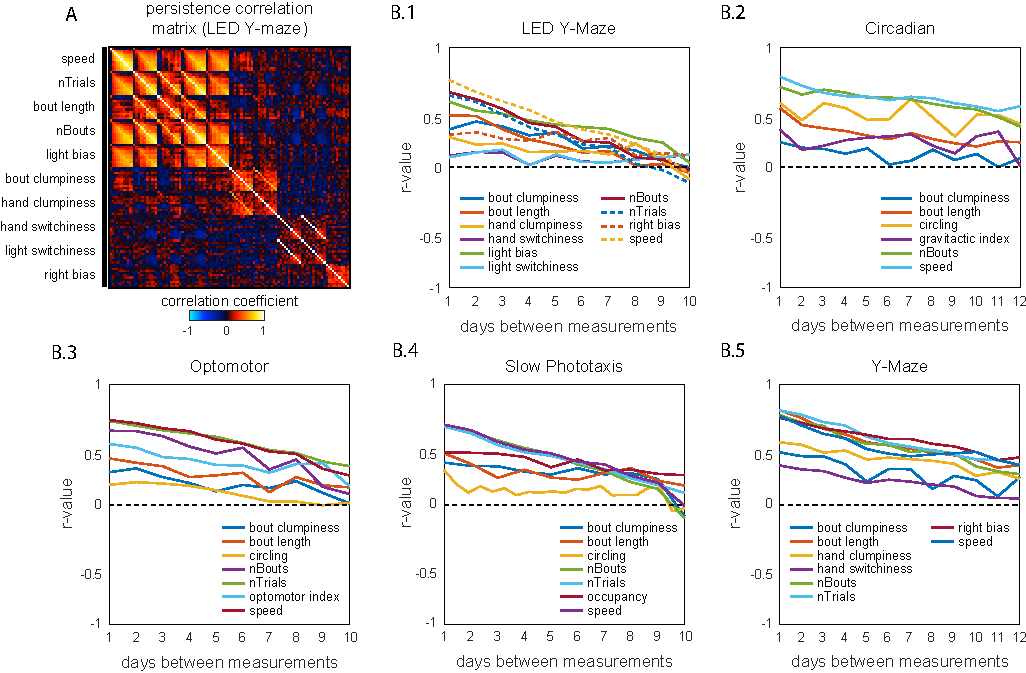
\includegraphics[width=\textwidth]{../figures/supplementary_figs/fig_s1.pdf}
    \vspace{.05in}
    \caption*{\textbf{Figure S1} — Caption.}
\end{figure}
\clearpage

% FIG S2 %
\begin{figure}[t!]
    \includegraphics[width=\textwidth]{../figures/supplementary_figs/fig_s2.pdf}
    \caption*{\textbf{Figure S2} — Caption.}
\end{figure}
\clearpage


% --- REFERENCES --- %
\section{References}

% references should be single spaced
\singlespacing
% insert bibliography from `dissertation.bib`
\bibliography{dissertation}

\end{document}




